\documentclass[sigconf]{acmart}

\usepackage{booktabs} % For formal tables
\usepackage{graphicx}
\graphicspath{ {img/} }

% Copyright
%\setcopyright{none}
%\setcopyright{acmcopyright}
%\setcopyright{acmlicensed}
\setcopyright{rightsretained}
%\setcopyright{usgov}
%\setcopyright{usgovmixed}
%\setcopyright{cagov}
%\setcopyright{cagovmixed}

% DOI
\acmDOI{10.475/123_4}

% ISBN
\acmISBN{123-4567-24-567/08/06}

%Conference
\acmConference[UMich'17]{EECS 549/SI 650}{April 2017}{Ann Arbor MI, USA} 
\acmYear{2017}
\copyrightyear{2017}

\acmPrice{Free}


\begin{document}
\title{Jarvis - A Smart Bot for Piazza}
\author{Pranav Ramarao, Isaac Bowen, Ke Yu}
\orcid{1234-5678-9012}
\affiliation{%
  \institution{University of Michigan}
  \city{Ann Arbor} 
}
\email{{pranavr, irbowen, yuke}@umich.edu}


% The default list of authors is too long for headers}
\renewcommand{\shortauthors}{Ramarao, Bowen, Yu}


\begin{abstract}
In this work, we explore some of the challenges faced with Piazza, specifically for large classes. We present a smart, interactive bot, Jarvis, that can tackle the problems by using state-of-the-art IR techniques. We show the Jarvis can greatly increase the efficiency of the instructors in managing large classes and also serve as a useful aid for students to master the material.
\end{abstract}

\keywords{IR, Piazza, search, similarity, FAQ generation, question answer system}

\maketitle
\section{Introduction}

\subsection{Piazza}
Piazza is a free online gathering place where students can ask and answer questions 24/7 under the guidance of their instructors. Collaboration occurs in real time, which encourages participation and fuels discussion. Students can ask questions, which fellow students and instructors can attempt to answer. Students can post questions, answers, and notes, publicly or anonymously. Instructors can post notes, answer student questions, endorse good questions and answers, and collect student feedback about this course. Piazza provide students participation report which help instructors to see students’ engagement in the class. Instructors can view the class report to see when in the term the most questions are being asked but not the other way around. Leading campuses across North America have a significant Piazza presence, especially for computer science courses. Larger courses typically have over 500 students getting involved in the feed

\subsection{Chat Bots}A chat bot is known as a computer program which conduct conversational question answering  with users in a certain domain or on a certain topic with natural language sentence.Such procedure is aiming at simulating a person’s behavior as a conversation partner and designed to pass the Turing test. Chat bots are commonly used in various dialog system for information acquisition and other customer services. Some natural language processing techniques are used in building chat bots.

\section{Problem}
Piazza is a great tool for students and instructors to interact with each other. It allows students to post questions on a class wide forum, where other students and instructors can answer the questions. For small classes, where the question volume is very low, the system works well. Instructors can respond quickly, and scale isn't an issue. However, as the departments grow and class sizes increase, it becomes difficult to answer all the questions in a timely manner. For our project, we wanted to focus on a few specific issues related to Piazza at scale. The authors are instructors for undergraduate courses at UofM - these course have roughly 400 and 600 students and only a handful of staff members to manage the class. We are interested in solving these problems to assists in our courses. We want to free up instructor's time so they don't have to spend all of their time answer questions on Piazza, and provide a better experience for students.

\subsection{Duplicate Questions}
As one of the side effects of the number of students posting questions, it becomes difficult for other students in the class to know if their question has already been asked. Given the question volume, they may not have time to read every question that is asked nor use the search facilities that piazza provides. As a result, students repost a question that is very similar to one that has already been asked. For instructors, this means that they have to answer the same question over and over, or link students to the previous question. This is not an easy task as a similar question might have been answered by another instructor which requires instructors to search in the first place. This requires instructors to know all of the questions that have been posted by all students, which clearly is not possible. For students, it could provide confusion, as many similar questions have very similar answers, but students are quite sure if its the same question (and therefore has the same answer). There is also the consistency issue where two instructors might not concur exactly on the duplicate questions which confuses students even more.

\subsection{Lack of a Weekly Summary}
A related issue is that students aren't getting the most they could out of Piazza because of the number of questions. Students can't dedicate hours every day to read through all questions posted every day. Also, many of the question are very student-specific (they won't relate to other students, so the whole class doesn't benifit from reading them). However, there are some questions that are very common, or exceptionally helpful, and it would be beneficial to aggregate these high quality questions. Ideally, students want to see a weekly report of 10 questions that they do not want to miss out on. This should allow students to get much more from Piazza, and allow them to use it as the interactive learning tool it was designed to be.

\subsection{Poor Search}
Piazza's search features leave something to be desired. The largest problem seems to be that the results are very heavily skewed towards the most recent results, when that may not actually be what the student is looking for. We wanted to provide a method for students to more accurately search Piazza for their questions (or answers), that isn't so heavily skewed by one factor. This feature will hopefully cut down on duplicate questions if it works well, as a good search feature should help students find questions similar to ones that have already been posted, so they can avoid posting duplicates.

\subsection{Information Retrieval}
How do we formulate the above problems as information retrieval problems?

Finding duplicate questions is a natural IR problem. We have to find the most similar posts in the collection, and then see if similarity score is above the threshold we have chosen. If so, we can flag this question as a duplicate.

Finding the top questions for the week for the FAQ is a question where both traditional IR techniques come into play, and we can use specific information made available from the Piazza platform.

Improve Piazza's search feature is directly an IR task. Piazza's search isn't very good at IR, and we want to make it better!

\begin{figure*}
\caption{A Piazza question, containing both a student and instructor answer. The highlighted boxes show some of the many features that we can extract from the post.}
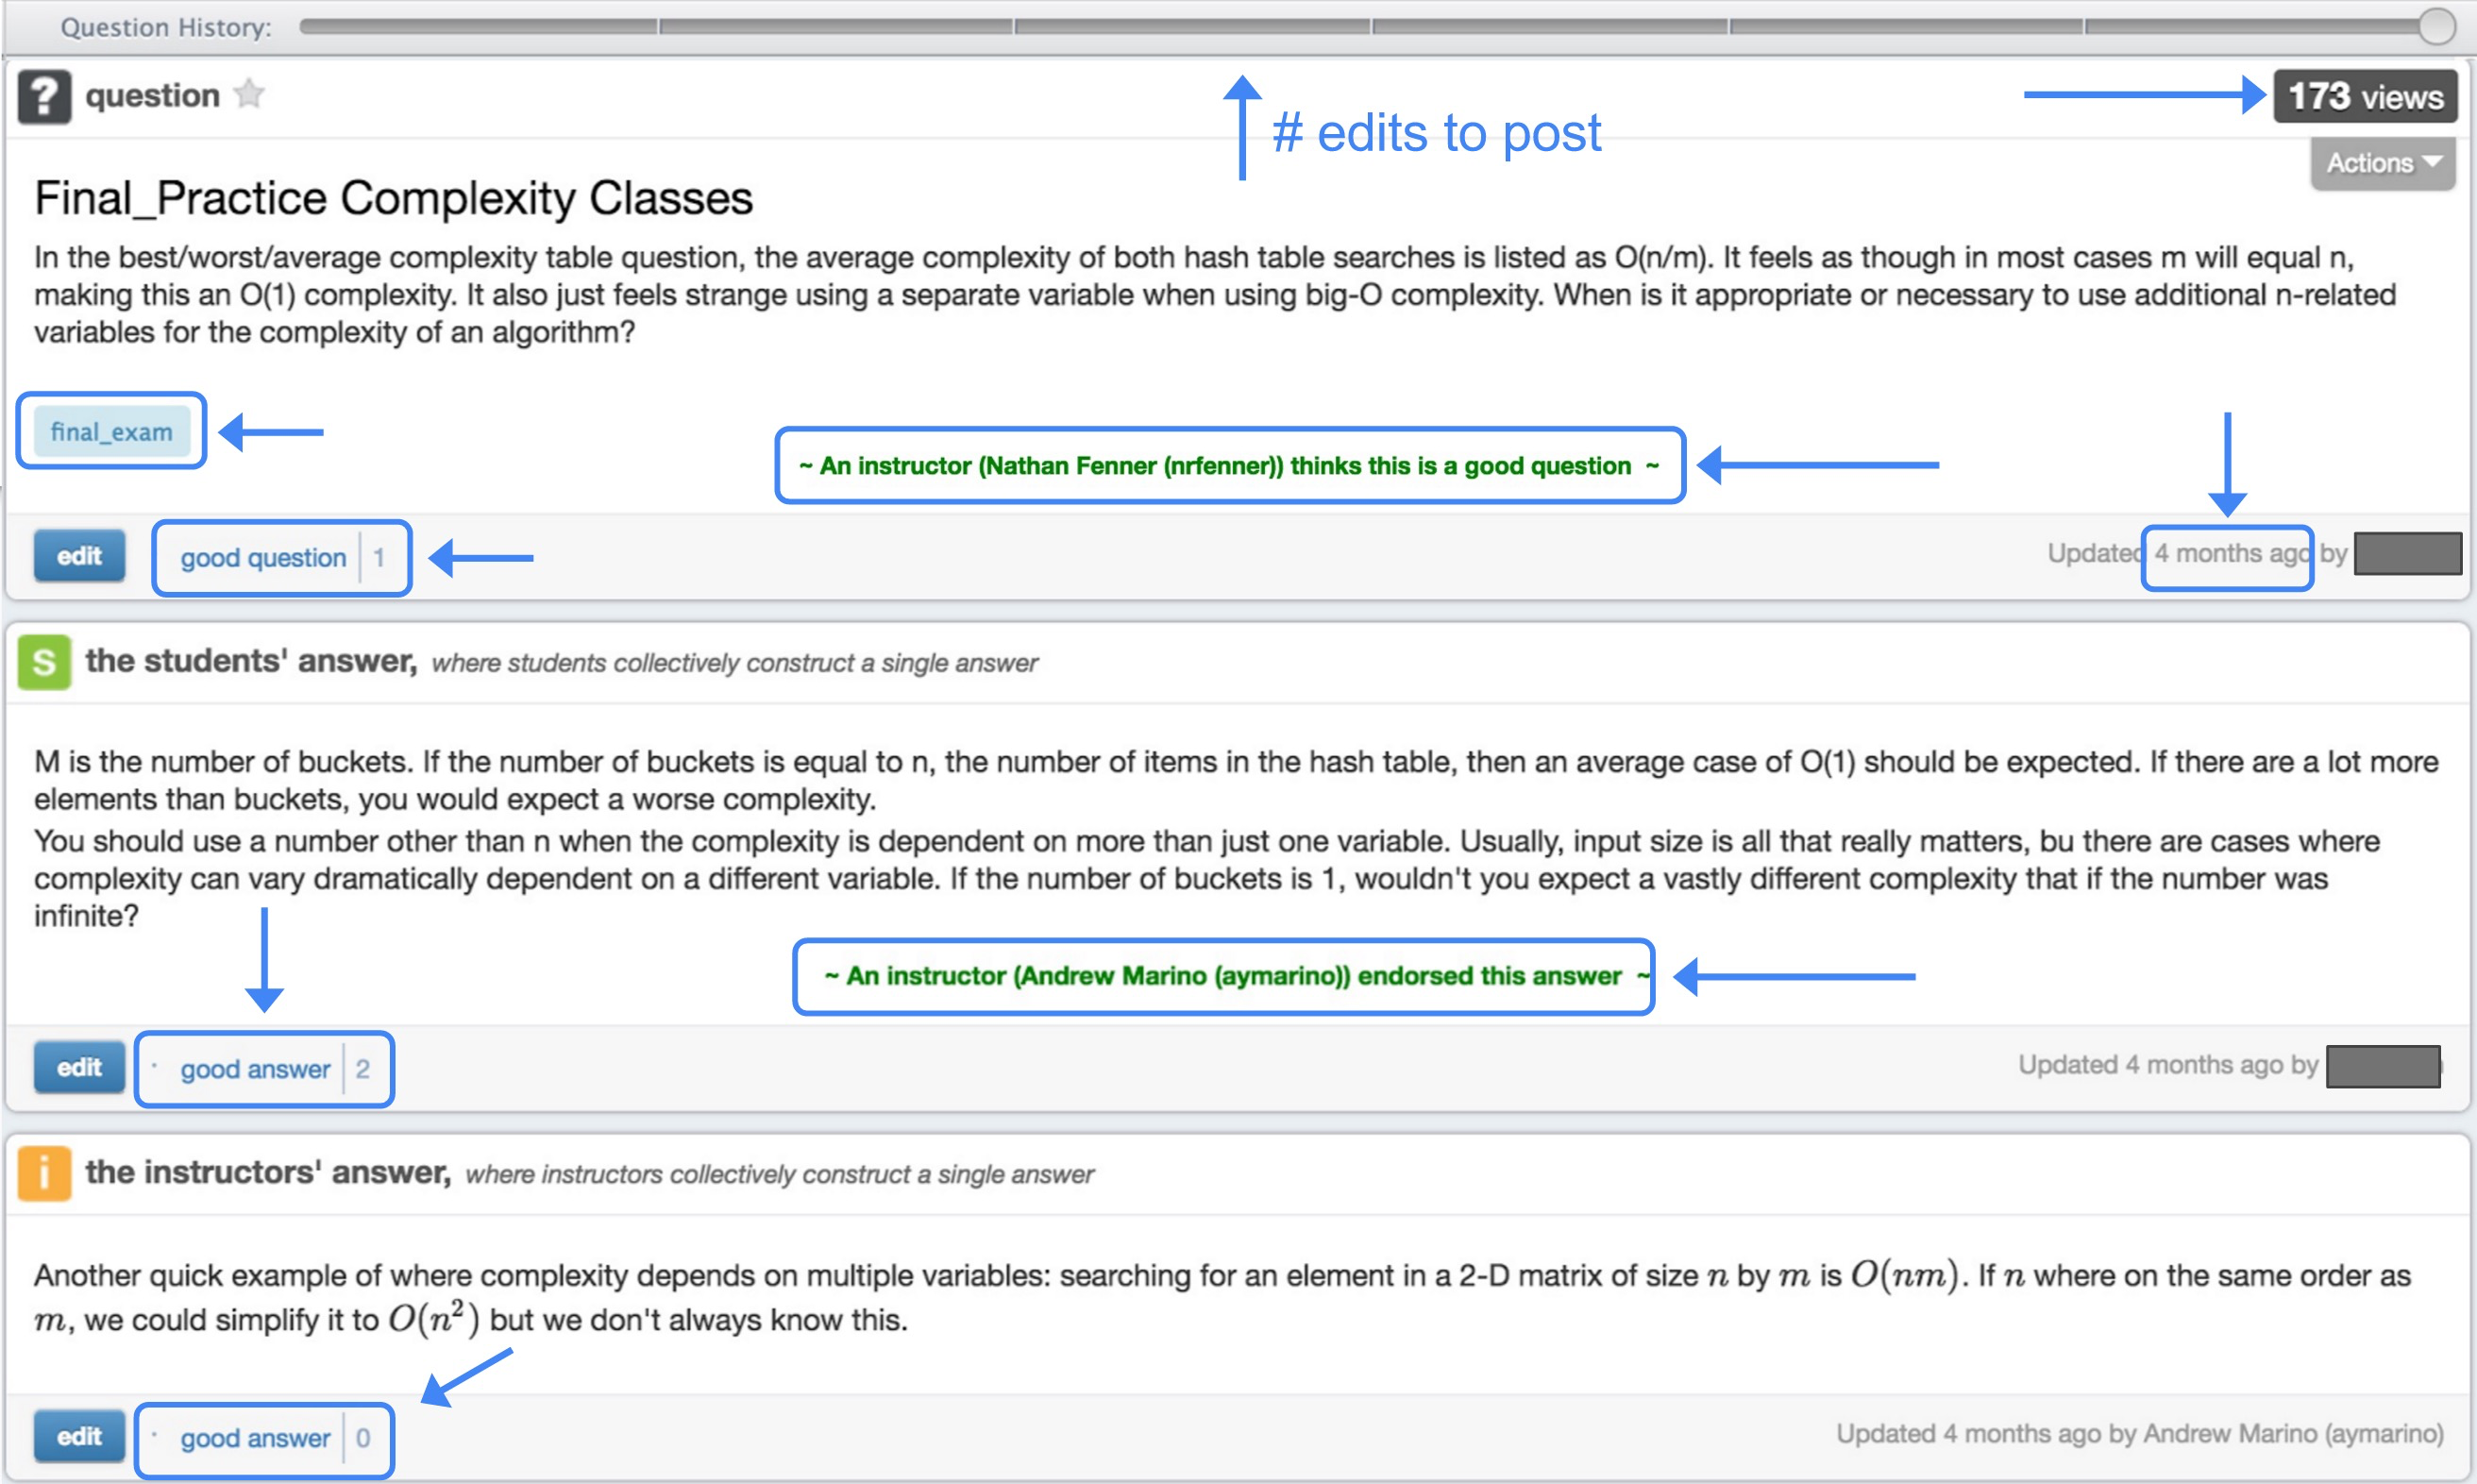
\includegraphics[width=\textwidth]{piazza_stats}
\end{figure*}

\section{Method}
We designed and implemented Jarvis, a bot written in python that can accomplish these goals. 

\subsection{System Overview}
Jarvis works by indexing all the contents of the course on Piazza. On start-up, it bulk downloads all of the questions and answers posted previously and constructs an index from there. After that, it periodically scrapes new contents and does an incremental update to the index.

\subsection{Tools and packages used}
We took advantage of several python packages and libraries to make the development of Jarvis smoother and more stable. We used python's whoosh library for indexing the documents. Whoosh is a full index library that supports many different operations - creating a schema, search index or certain columns, quick searches (using BM25) and also date range queries. 

\subsection{Data Crawling}
Piazza does not provide an elegant or easy way to programmatic-ally interact with its posts. To get the questions and answers on the site, we had to use an unofficial API. This API has been reversed engineered [*insert reference*] and most of the actions that one can perform on the piazza website can be done through the API. We started from this API, and then built our own abstraction on top of it that would read in posts and then store them in our whoosh on disk index. To speed up processing, testing, and to prevent Piazza from potentially rate limiting us, we also developed a feature to bulk download and store course data, which we could then treat as our "Piazza" input data for indexing and pre-processing purposes. We extracted several past semesters of the course EECS 281, and were able to use that as our training set.


\subsection{Feature Extraction}
The raw data that we get through the APIs aren't fully sufficient for the purposes of our bot. For instance, we require features such the \# of endorsements from students and the instructors separately since they help in improving the quality of results. We also define a feature 'activity score' of a post which looks at the number of updates made to a post, the number of student and instructors involved, and also the number of follow-ups in the post.

\subsection{Data Preprocessing}
The subject and body of the post in its raw form is HTML format. We remove all the irrelevant HTML tags from the post body. We concatenate the title with the body together to make it easier for searching purposes.For each document, we perform some basic text cleaning by removing special characters through regex and also convert all text to lowercase.We also remove the stop words from documents and apply Porter stemmer [Porter, Martin F. "Snowball: A language for stemming algorithms." (2001).] from nltk[Bird S. NLTK: the natural language toolkit[C]//Proceedings of the COLING/ACL on Interactive presentation sessions. Association for Computational Linguistics, 2006: 69-72.] package to further shrink the vocabulary size. 

\subsection{Duplicate Detection}
We implemented a function called find\_top\_N\_similar\_docs(), which achieve following functionality: input a new post, and a collection of existing posts, and a integer n, we can return the top n posts with highest similarity scores against new input post. 

By representing the text document using vector space model, we can calculate relevance between the documents. Before that, for the term selection, we calculated the TF* IDF(term frequency–inverse document frequency) score for each words in documents by using sklearn built-in function. And then calculate the similarity between new posted documents with all documents in the whole collection. The posts on piazza usually are more than 5 words long, and we consider the document not short yet not too long. In this case, Cosine similarity measure or Dice similarity measure would be more efficient since these measures tend not to over penalize non-overlapping terms. In our implementation, we used Cosine similarity measure for reliability. By comparing pair-wise similarity scores of new input post and all posts in the collections  with input parameters N, we can return top N most similar documents with highest scores in the collections. 


\subsection{Top Questions}
Every week on a Sunday, Jarvis makes an attempt to post the top 10 questions that could be relevant for every student in the course. To do this, Jarvis retrieves all the posts made one week prior to that Sunday from the whoosh index. Posts that do not contain an instructor answer are filtered out since they would not be of much use. With the remaining posts, Jarvis looks at various features of the posts and scores them. The key features that contribute to the score are :

\begin{enumerate}
  \item \# good question endorsements
  \item \# good question endorsements by TAs
  \item \# good answer endorsements
  \item \# good answer endorsements by TAs
  \item \# unique views
  \item \# student follow-ups
\end{enumerate}

For each of the above features, we assign weights based on their importance. We finally rank the results and then return the top 10 results. We also threshold the scores so that during dry weeks, we don't return stale/irrelevant posts.

\subsection{Improved Search Feature}
For the search task, we are able to improve upon piazza's search facility in the following ways:
\begin{enumerate}
\item treat recency as a metric
\item support typos made in query
\item OR based query on each term rather than AND based one
\item importance to finding query term on subject/body rather than answer
\end{enumerate}

A recency based search has the issue of having important posts go down the search results. We make recency as one of the features among the others. We use a decay function to make sure that old posts don't get a very low score. From our experience, typically posts which are older than a month get the same recency score. We run the query through a spell correction engine which replaces query terms when a high confidence is present. We do not perform an AND based search as sometimes, students include an extra term which returns no results. Hence, we score results that are able to match all terms more, but when no post matches all terms, we see the number of terms matched and also the maximum n-gram match for the query. 

\section{Results}
Here we present the results of our system.
To test our system, we set up a mock Piazza course where we could post fake questions to Jarvis. Jarvis has read only access to previous semesters of questions, and read/write access on the mock course. When new questions are posted, Jarvis can read those questions, and write answers to them, but it cannot write to the past semesters course.

\subsection{Duplicate Detection}
To test our system, we found all questions in previous semesters that had been marked with an '@'. This means that an instructor read the question, and decided that it was similar enough to a previous question, that, instead of answering it, they decided to simply link to a previous question. We used this set of questions to test our system. We found that our system performed very well on this data set, responding to more than 90 percent of known duplicate posts correctly.

Perhaps more exciting is the fact that our system was able to identify some duplicate questions that instructors did not find themselves. When we fed our system questions that specifically had not been marked with an '@', we found that some of them were still marked by our bot. Many of these were, in fact, duplicates that had been answered twice, by two separate instructors at two separate occasions. However, since this data is not labeled, there is no easy way for us to determine our systems efficacy without looking at every duplicate it flags and checking to see if it seems logical. For the vast majority of the new duplicates flagged by our system, it seems to work well.

\subsection{Top Questions}
Jarvis's default behavior is to simply sit in a while loop, waiting for new questions to be posted. However, it can be instructed to create a special post on Piazza, containing the top questions for a certain week.

Jarvis will then look through all of the questions that have been posted in the given time frame, and extract a variety of features from the questions. Based on these combinations of features, Jarvis will assemble as list of the top 10 (TODO FIX ME FIVE TEN WHAT?) questions posted. 

Unfortunately, 'best' or 'top' questions is an extremely subjective measure. We do not have a golden list of the best questions to compare our results to. So, we tried to do a few things. We looked through several weeks worth of questions, and tried to find a few, extremely important posts that we knew \textit{must} show up in the final output. These included instructor clarification posts, notes about when and where the exams were, and other important course logistic posts. For the questions we found, Jarvis always had these in the top ten. The other way we were able to evaluate is by manually looking at the questions that Jarvis has found, and attempt to determine if the questions reflect the best questions posted that week. Again, this was extremely subjective, but for every question listed in the top questions, we were able to find something about it that made it worthy of being in the list.

\subsection{Better Search Features}
To take advantage of our improved tag feature, students can post private questions with their search query, under a specific tag. When Jarvis sees questions that are posted with this tag, it searches for all similar questions and responds to the post with links to the most similar questions. While this is a more involved process then using the built in search feature in Piazza, we feel that the improved accuracy of the results is worth the additional time investment.

To evaluate our search results, we prepared a list of posts that we were looking for, and some keyword queries to try to locate those posts. We found that, when the post we were looking for was very recent, our improved search did not perform any better than the built in search. However, this is expected, as Piazza's search feature is heavily skewed towards the most recent posts. Once we searched for posts that were further in the past, our system performed much better. Unfortunately, since we are trying to improve on Piazza's ranking, we cannot use there results as a source of truth against which to calculate Kendalls Tau or other useful metrics. Therefore, most of our measurements were extremely subjective, and involved entering in identical queries into both systems and manually comparing the results. The results returned were almost always the same, but our results ranked the documents we were actually looking for much higher than Piazza's default search.

\section{Discussion}

\subsection{Conclusion}
We design and implemented Jarvis bot, a python implementation of a chat bot meets information retrieval system that allows us to more effectively manage Piazza with large classes.
TODO TODO TODO TODO

\subsection{Deliverables}
We have open-sourced on implementation of Jarvis, as well as the code to download and index Piazza. All of the Jarvis bot code is available on Github, \href{https://github.com/pranavr93/piazza_bot}{here}

\subsection{Lessons Learned}
A large portion of our work had to do with dealing with messy input data scraped from Piazza. Because the API is unofficial, there were many additional steps that we had to take before we had a clean dataset of questions and answers for each course. 

We have learn how to use existing natural language processing packages to avoid implement basic algorithms from scratch. More importantly, whatever a library is omnipotent, we have to modify it to suit our need. Thus, the importance of a solid foundation in understanding the whole process and every tiny detail of the design would be never be exaggerated. 

I'm sure we learned some other things. 
TODO TODO TODO TODO

\subsection{Future Work}
In the future, we can improve our algorithm by improving on term selection and similarity calculation. For term selection, we can improve by using n-gram, for example bi-gram or trigram, which may better capture the relationship in each document.Also, we could try implement  grammar structure analysis of a sentence using a set of input transformation rules to represent grammar rules. For similarity calculation, we can try applying different similarity functions and use cross validation to find a better model. Besides, we could also try to applying applying new techniques, for example word2vec, to reduce the calculation.

To improve our weekly Top Questions feature, we have a few plans. For one, we want to expand, so that we aren't just looking at questions, but also answers. It is entirely possible that many different questions all have the same common problem, and are given a common answer. It would be great for our FAQ to be able to list these very common answers, and all of the questions that they are associated with.

A goal that is a bit more far-fetched, but certainly within the realm of possibility, is to actually add full question answering to Jarvis. Jarvis could look at recently posted questions, and instead of simply linking to a previous post, it could try to answer the question. This would involved adding new layers to Jarvis, but the infrastructure is set up to be easy to expand.

more TODO TODO TODO TODO



\bibliographystyle{ACM-Reference-Format}
\bibliography{sigproc} 

\end{document}
